\section{Introduction}
There are two predominate methods for predicting global bathymetry in use today.  
The Smith and Sandwell method \cite{sandwell}, and physical collection by survey ships through the use of varying types of sonar.  
The Smith and Sandwell method uses satellite imagery to estimate the mass of seamounts.

\begin{figure}[hb]
    \centering
    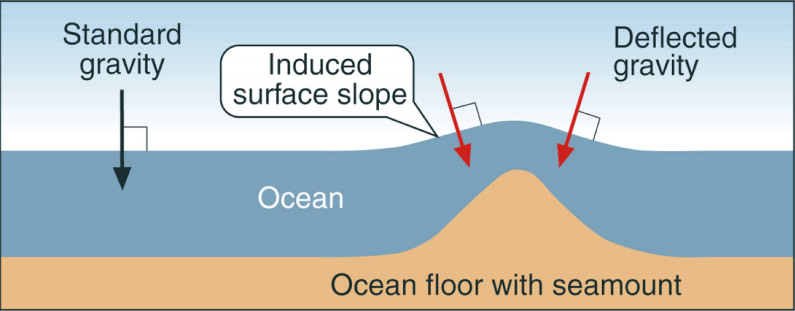
\includegraphics[scale=0.25]{mountainAltimetry}
    \caption{Graphic showing the Smith and Sandwell method}
    \label{fig1:Figure 2}
\end{figure}

\par
This method has known accuracy issues and can be hindered by the presence of clouds and ice formations. 
While not the most accurate solution, satellite calculations provide a mechanism for producing coarse approximations of bathymetry in locations that physical collection is not allowed or ideal. 
The most approximate way to determine bathymetry is through sonar depth soundings. 
Today, ships equipped with sonar, can measure the depth of a given area with great precision.  
While precise, it is not practical to survey the entire globe for bathymetry.  
Constraints to this approach are cost, time, and international law restricting the use of certain maritime areas.

\par
To address these issues the Naval Research Laboratory (NRL) has proposed a research project titled “Predicting Global Altimetry” lead by geophysicist Dr. Warren Wood. 
The goal of this project is to develop models that will accurately predict world-wide bathymetry.  
The method being employed is to use machine learning to train algorithms on different sets of input parameters, for different scenarios, to produce higher resolution bathymetry.  
The input parameters these algorithms require come from multiple sources, but for the scope of this project we will focus on the ones that are calculated from existing datasets.  
It is NRL’s hypothesis that derived statistical data from existing gridded bathymetric data sets can be used as training data to increase prediction accuracy.